\providecommand{\addcausa}[2]{
    node[punto, pos=#1] {} node[causa, left=0.1cm, pos=#1] {#2}
}

\providecommand{\espina}[5]{
    \node[categoria] (#1) at ([shift={(-1.5, #3)}] #2) {#4};
    \draw[thick, ->] (#1) -- (#2) #5;
}
% ------------------------------------------

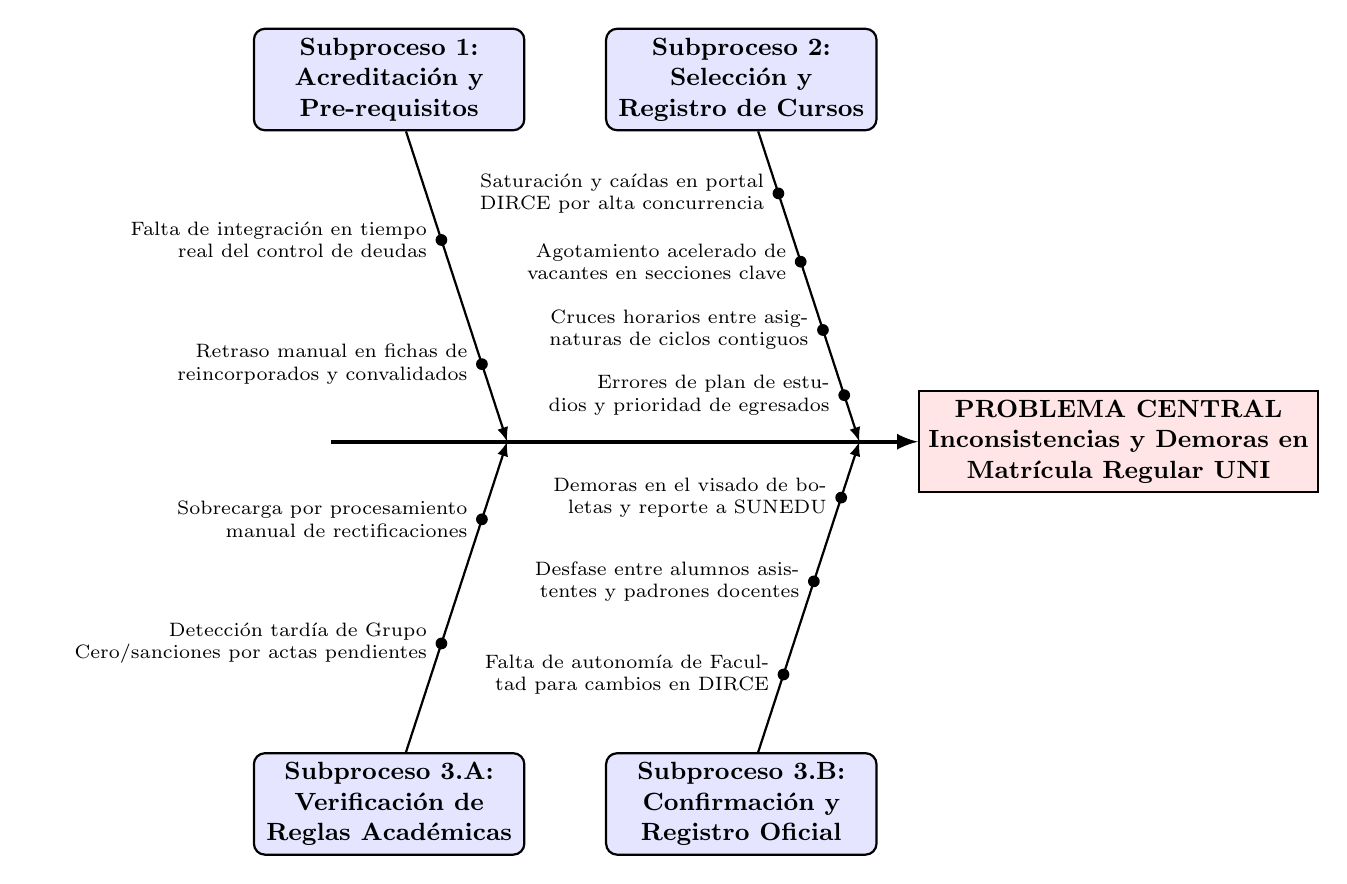
\begin{tikzpicture}[
    >=latex, thick,
    efecto/.style={draw, rectangle, fill=red!10, minimum width=3.8cm, minimum height=1.2cm, align=center, font=\bfseries\small},
    categoria/.style={draw, rectangle, fill=blue!10, rounded corners, text width=3.2cm, align=center, font=\bfseries\small},
    causa/.style={draw=none, inner sep=2pt, font=\scriptsize, align=right, text width=5cm}, 
    punto/.style={circle, fill=black, inner sep=1.5pt}
]

    % EJE CENTRAL Y PROBLEMA CENTRAL
    \node[efecto] (P) at (10,0) {PROBLEMA CENTRAL\\Inconsistencias y Demoras en\\Matrícula Regular UNI};
    \draw[ultra thick, ->] (0,0) -- (P);

    % PUNTOS DE CONEXIÓN EN EL EJE CENTRAL
    \path (0,0) -- (P.west)
        coordinate[pos=0.3] (S1)
        coordinate[pos=0.9] (S2);

    % ESPINAS SUPERIORES
    \espina{SUB1}{S1}{4.6}{Subproceso 1:\\Acreditación y\\Pre-requisitos}{
        \addcausa{0.35}{Falta de integración en tiempo real del control de deudas}
        \addcausa{0.75}{Retraso manual en fichas de reincorporados y convalidados}
    }

    \espina{SUB2}{S2}{4.6}{Subproceso 2:\\Selección y\\Registro de Cursos}{
        \addcausa{0.20}{Saturación y caídas en portal DIRCE por alta concurrencia}
        \addcausa{0.42}{Agotamiento acelerado de vacantes en secciones clave}
        \addcausa{0.64}{Cruces horarios entre asignaturas de ciclos contiguos}
        \addcausa{0.85}{Errores de plan de estudios y prioridad de egresados}
    }

    % ESPINAS INFERIORES
    \espina{SUB3A}{S1}{-4.6}{Subproceso 3.A:\\Verificación de\\Reglas Académicas}{
        \addcausa{0.35}{Detección tardía de Grupo Cero/sanciones por actas pendientes}
        \addcausa{0.75}{Sobrecarga por procesamiento manual de rectificaciones}
    }

    \espina{SUB3B}{S2}{-4.6}{Subproceso 3.B:\\Confirmación y\\Registro Oficial}{
        \addcausa{0.25}{Falta de autonomía de Facultad para cambios en DIRCE}
        \addcausa{0.55}{Desfase entre alumnos asistentes y padrones docentes}
        \addcausa{0.82}{Demoras en el visado de boletas y reporte a SUNEDU}
    }

\end{tikzpicture}